% =============================================================================
%  Breadcrumbs
%  Blockchain Olympiad submission, Team CookieMonsters, United International
%  University.
%
%  HOW TO COMPILE
%    Upload main.tex and ref.bib to Overleaf. Set the compiler to pdfLaTeX.
%    Overleaf runs BibTeX automatically. Nothing else is needed: every figure
%    is drawn in TikZ inside this file, so there are no image files to upload.
%
%  >>> EDIT THE TEAM BLOCK BELOW BEFORE SUBMITTING <<<
% =============================================================================
\documentclass[11pt,border=6pt,varwidth=20cm]{standalone}

% ---- team details: replace the bracketed placeholders -----------------------
\newcommand{\TeamName}{CookieMonsters}
\newcommand{\TeamInstitution}{United International University, Dhaka, Bangladesh}
\newcommand{\TeamMembers}{Ahbab, Ruhi, Rohan, Ishmam, Adnan}
\newcommand{\TeamCategory}{Undergraduate}
\newcommand{\TeamContact}{mkhan223869@bscse.uiu.ac.bd}
% -----------------------------------------------------------------------------

\usepackage[T1]{fontenc}
\usepackage[utf8]{inputenc}
\usepackage{lmodern}

\usepackage{amsmath,amssymb}
\usepackage{graphicx}
\usepackage{xcolor}
\usepackage{booktabs}
\usepackage{tabularx}
\usepackage{array}
\usepackage{longtable}
\usepackage{caption}
\usepackage{enumitem}
\usepackage{titlesec}

\usepackage{tikz}
\usepackage{pgfplots}
\usepackage{algorithm}
\usepackage{algpseudocode}



\usetikzlibrary{positioning,shapes.geometric,arrows.meta,calc,fit,backgrounds}
\pgfplotsset{compat=1.18}

% ---- palette (colour-blind safe, prints correctly in greyscale) -------------
\definecolor{tcblue}{HTML}{2563EB}
\definecolor{tcorange}{HTML}{E8710A}
\definecolor{tcgreen}{HTML}{059669}
\definecolor{tcgrey}{HTML}{6B7280}
\definecolor{tctext}{HTML}{111827}
\definecolor{tcline}{HTML}{E5E7EB}
\definecolor{tcbg}{HTML}{F7F8FA}


\captionsetup{font=small,labelfont={bf,sf}}
\setlength{\parskip}{0.35em}
\renewcommand{\arraystretch}{1.18}




\newcolumntype{Y}{>{\raggedright\arraybackslash}X}
\newcommand{\est}{\textsuperscript{\textdagger}}

% ---- the logo, drawn rather than imported ----------------------------------
% A trail of marks, each one larger and more definite than the last, ending in
% the verified record. Drawn rather than imported so the file stays standalone.
\newcommand{\bclogo}[1][1.0]{%
\begin{tikzpicture}[scale=#1,every node/.style={transform shape}]
  \node[regular polygon,regular polygon sides=6,draw=tcblue,line width=1.5pt,
        minimum size=2.35cm,rotate=90] (hex) at (0,0) {};
  \draw[tcgrey!45,line width=1.0pt,dash pattern=on 1pt off 2.6pt,line cap=round]
        (-0.53,-0.36) -- (0.53,0.36);
  \fill[tcgrey!55] (-0.53,-0.36) circle (0.085);
  \fill[tcgrey]    (-0.27,-0.17) circle (0.110);
  \fill[tcblue]    ( 0.00, 0.00) circle (0.135);
  \fill[tcorange]  ( 0.27, 0.17) circle (0.155);
  \fill[tcgreen]   ( 0.53, 0.36) circle (0.180);
\end{tikzpicture}}

\begin{document}
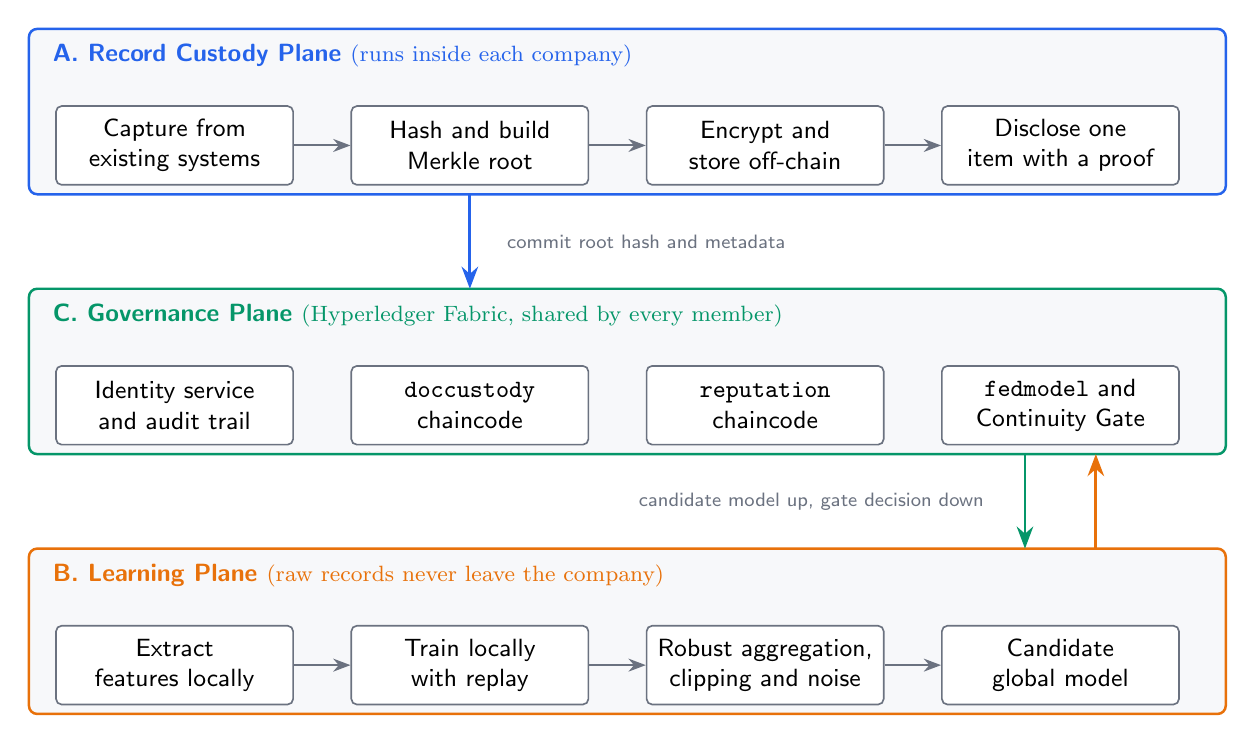
\begin{tikzpicture}[
  font=\sffamily\small,
  box/.style={rounded corners=2pt,draw=tcgrey,fill=white,line width=0.6pt,
              minimum height=1.0cm,text width=2.8cm,align=center,inner sep=3pt},
  band/.style={rounded corners=3pt,line width=0.9pt},
  lbl/.style={font=\sffamily\bfseries\small,align=left},
  ar/.style={-{Stealth[length=2.8mm]},line width=1.0pt},
  flow/.style={-{Stealth[length=2.2mm]},line width=0.7pt,tcgrey},
  tag/.style={font=\sffamily\scriptsize,text=tcgrey}]

% ---- Plane A: record custody (top) ----
\fill[tcbg,band,draw=tcblue] (0,7.0) rectangle (15.2,9.1);
\node[lbl,anchor=north west,text=tcblue] at (0.18,9.03)
  {A. Record Custody Plane \normalfont\footnotesize(runs inside each company)};
\node[box] (a1) at (1.85,7.62) {Capture from existing systems};
\node[box] (a2) at (5.60,7.62) {Hash and build Merkle root};
\node[box] (a3) at (9.35,7.62) {Encrypt and store off-chain};
\node[box] (a4) at (13.10,7.62) {Disclose one item with a proof};
\draw[flow] (a1) -- (a2); \draw[flow] (a2) -- (a3); \draw[flow] (a3) -- (a4);

% ---- Plane C: governance (middle, because it mediates the other two) ----
\fill[tcbg,band,draw=tcgreen] (0,3.7) rectangle (15.2,5.8);
\node[lbl,anchor=north west,text=tcgreen] at (0.18,5.73)
  {C. Governance Plane \normalfont\footnotesize(Hyperledger Fabric, shared by every member)};
\node[box] (c1) at (1.85,4.32) {Identity service and audit trail};
\node[box] (c2) at (5.60,4.32) {\texttt{doccustody} chaincode};
\node[box] (c3) at (9.35,4.32) {\texttt{reputation} chaincode};
\node[box] (c4) at (13.10,4.32) {\texttt{fedmodel} and Continuity Gate};

% ---- Plane B: learning (bottom) ----
\fill[tcbg,band,draw=tcorange] (0,0.4) rectangle (15.2,2.5);
\node[lbl,anchor=north west,text=tcorange] at (0.18,2.43)
  {B. Learning Plane \normalfont\footnotesize(raw records never leave the company)};
\node[box] (b1) at (1.85,1.02) {Extract\\features locally};
\node[box] (b2) at (5.60,1.02) {Train locally with replay};
\node[box] (b3) at (9.35,1.02) {Robust aggregation, clipping and noise};
\node[box] (b4) at (13.10,1.02) {Candidate global model};
\draw[flow] (b1) -- (b2); \draw[flow] (b2) -- (b3); \draw[flow] (b3) -- (b4);

% ---- cross-plane couplings: short, vertical, in the gaps ----
\draw[ar,tcblue] (5.60,7.0) -- (5.60,5.8);
\node[tag,anchor=west] at (5.95,6.40) {commit root hash and metadata};

\draw[ar,tcorange] (13.55,2.5) -- (13.55,3.7);
\draw[ar,tcgreen]  (12.65,3.7) -- (12.65,2.5);
\node[tag,anchor=east] at (12.25,3.10) {candidate model up, gate decision down};
\end{tikzpicture}
\end{document}
